\documentclass[b5paper,openany]{standalone}
\usepackage{luatexja-preset}
\usepackage{xcolor}
\usepackage{tikz}
\usetikzlibrary{calc}

\begin{document}
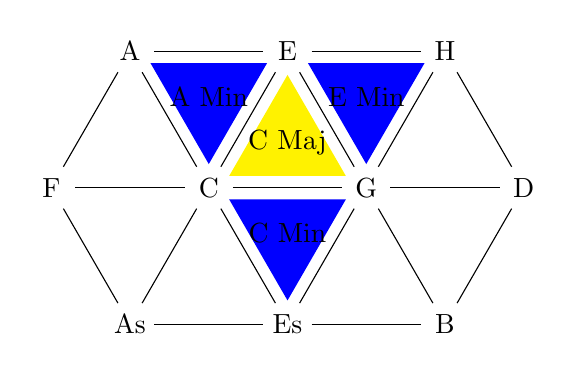
\begin{tikzpicture}[scale=2]
  \tikzset{every node/.style={shape=circle,text centered,inner sep=0pt,minimum size=0.6cm}};
  \node (T) at (0,0){C};
  \node (D) at (1,0){G};
  \node (S) at (-1,0){F};
  \node (M) at (60:1){E};
  \node (SM) at ($(S)+(M)$) {A};
  \node (m) at (-60:1){Es};
  \node (Sm) at ($(S)+(m)$) {As};
  \node (DD) at ($(D)+(D)$) {D};
  \node (DM) at ($(D)+(M)$){H};
  \node (Dm) at ($(D)+(m)$){B};
  \fill[yellow] ($(T.center)+(30:0.15)$)--  ($(D.center)+(150:0.15)$)--  ($(M.center)+(270:0.15)$)--cycle;
  \fill[blue]   ($(M.center)+(-30:0.15)$)-- ($(DM.center)+(-150:0.15)$)--($(D.center)+(-270:0.15)$)--cycle;
  \fill[blue]   ($(SM.center)+(-30:0.15)$)--($(M.center)+(-150:0.15)$)-- ($(T.center)+(-270:0.15)$)--cycle;
  \fill[blue]   ($(T.center)+(-30:0.15)$)-- ($(D.center)+(-150:0.15)$)-- ($(m.center)+(-270:0.15)$)--cycle;
  \draw (S) -- (T) -- (D) -- (DD);
  \draw (SM) -- (M) -- (DM);
  \draw (Sm) -- (m) -- (Dm);
  \draw (S)--(SM)--(T)--(M)--(D)--(DM)--(DD);
  \draw (S)--(Sm)--(T)--(m)--(D)--(Dm)--(DD);
  \node (CMaj) at ($0.334*(T) +0.333*(D) +0.333*(M)$){C Maj};
  \node (EMin) at ($0.334*(DM)+0.333*(D) +0.333*(M)$){E Min};
  \node (AMin) at ($0.334*(T) +0.333*(SM)+0.333*(M)$){A Min};
  \node (CMin) at ($0.334*(T) +0.333*(D) +0.333*(m)$){C Min};
% \draw[red,font=\tiny,arrows={->}] (DM) -- (T) node[midway,sloped,above]{lead-tone};
% \draw[red,arrows={->}] (D) to[bend left] (T);
% \draw[blue,font=\tiny,arrows={->}] (Sm) -- (D) node[midway,sloped,above]{inv.~lead-tone};
% \draw[blue,arrows={->}] (S) to[bend left] (T);
\end{tikzpicture}
\end{document}
